%
% Copyright (C) 2011 Agostino De Marco
%                    <agostino dot demarco at unina dot it>
%                    Roberto Giacomelli
%                    <giaconet dot mailbox at gmail dot com>
%
%    This work may be distributed and/or modified under the
%    conditions of the LaTeX Project Public License, either
%    version 1.3 of this license or any later version.
%    The latest version of this license is in
%    http://www.latex-project.org/lppl.txt and version 1.3
%    or later is part of all distributions of LaTeX version
%    2005/12/01 or later.
%
% This work has the LPPL maintenance status `maintained'.
% 
% The Current Maintainer of this work are Agostino De Marco
% and Roberto Giacomelli
%
\documentclass{standalone}
\usepackage{lmodern}
\usepackage{pgfplots}

\begin{document}
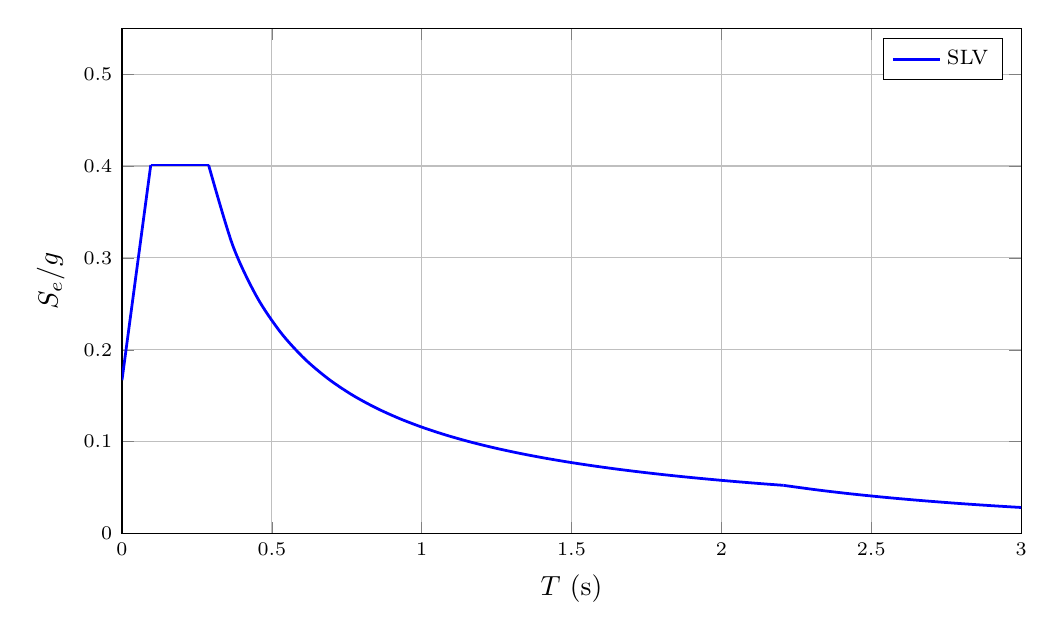
\begin{tikzpicture}
% defining personal drawing style
\pgfplotsset{
  slv/.style={line width=1pt,color=blue},
}

\begin{axis}[
   % etichette del grafico
     tick label style={font=\scriptsize},
     xlabel={$T$ (s)},
     ylabel={$S_e/g$},
     xtick={0,0.5,...,3.0},
     grid=major,
   % linee di plottaggio
     no markers,
   % dominio 2D
     smooth,
     xmin=0, xmax=3.00,
     ymin=0, ymax=0.55,
   % dimensioni tela
     width=13cm,
     height=8cm,
   % variabile nelle espressioni: periodo T
     variable=\T
    ]

\def\ag{0.15182}
\def\Fo{2.402}
\def\Ss{1.10}
\def\Tb{0.096}
\def\Tc{0.289}
\def\Td{2.207}

\addplot[slv,domain=0.0:\Tb]
   {\ag*\Ss*\Fo*(T/\Tb+(1/\Fo)*(1-T/\Tb))};
\addplot[slv,domain=\Tb:\Tc]
   {\ag*\Ss*\Fo};
\addplot[slv,domain=\Tc:\Td]
   {\ag*\Ss*\Fo*\Tc/T};
\addplot[slv,domain=\Td:5.0]
   {\ag*\Ss*\Fo*\Tc*\Td/T^2};

% legenda
\legend{\textsc{slv},,,}
\end{axis}
\end{tikzpicture}
\end{document}



